\section{Secure Group Communication}
The most sophisticated approach to the scalability problem is to create a secret \textit{group key} (\ac{GK}) each time multiple devices need to access the same file. This schemes are called "Secure Group Communication" (\ac{SGC}). The main idea is to reduce the number of filekeys by encrypting all files with a unique \ac{GK} that is only known to the members in the share. Simple approaches use a so called \textit{Key Distribution Center} (\ac{KDC}) to distribute the group keys to each member. However, while Bdrive could manage forward secrecy quite easily, this schemes suffer from additional reencryption overhead if a member leaves the group. 

% Mutlicast in group communications
Commonoly Secure Group Communications are mentioned together with \textit{multicast messages}. With multicast the same message is distributed to different devices in one setting. In contrast stands \textit{unicast}. Here a central authority is required that manages authentication and authorization to decide which entity should access which content. With multicast messages, however, content is distributed to each entity regardless if this entity is authorized to access this content. Instead authorization is handled via encryption of the content. If an entity owns the key to decrypt the data it is implicitly authorized to access the content as well. Multicast messages are especially handy in group communications since they only need to send one message to distribute the information to all members. As a the trade-off the message size increases.

% The role of \ac{PKI} in group communications
While there are many approaches researching secure group communication and making the rekeying process more efficient, the number of schemes can be reduced to those applicable to secure could storage. Here some prerequisites are given that are not generally assumed. Secure cloud storage system often deploy a public key infrastructure (\ac{PKI}) to bind identities to public keys of clients which means that a key exchange already happened.

In contrast to that are schemes that extend the 2-parties Diffie-Hellman (\ac{DH}) key exchange to n-party scheme, such as in \textit{Steiner at. al., 1996}\cite{steiner1996diffie}. The \ac{DH} key exchange is designed for unsecured environments to create a unique communication key, known to every member in the group, but not known to a passive attacker. However, since all communication is already disclosed and secured by the \ac{PKI} those schemes can be eliminated. They suffer from additional computation or message exchange overhead compared to schemes that assume an existing \ac{PKI}.   

In the following it is widely assumed that a client is identified uniquely by its public key, which is also known by the cloud server and can be queried by other clients. 

\subsection{Group Key Management Protocol}
The Group Key Management Protocol (\ac{GKMP})\cite{harney1997group} addresses the rekeying problem in a simple but scalable way. If a device want to share files with a group of other clients it creates the group key and encrypts all filekeys with this group key. This \ac{GK} needs to be securely distributed to all members which means that the data owner needs to download and store every public key of the group members and encrypt the \ac{GK} for each of them. Further, the data owner needs to encrypt all shared filekeys symmetrically with the chosen group key. 

% Disadventage
To ensure forward secrecy, the \ac{GK} needs to be renewed every time a member leaves the group. This overhead is located in the same computational magnitude as bootstrapping a new group. 

% Adventage
The big advantage of this scheme, compared to the scheme employed in Bdrive, is that it reduces the overhead of the number of encryptions, messages and keys on new file upload dramatically. While the data owner had to create a filekey for each member respectively, \ac{GKMP} reduces this to one filekey per upload. Additionally, since no backward secrecy have to be ensured, the \ac{GK} only have to be distributed to the new member\footnote{With backward secrecy the GK would have been renewed each time a new member joins.}.

\subsection{Logical Key Hierarchy}
\begin{figure*}[!ht]
\centering
    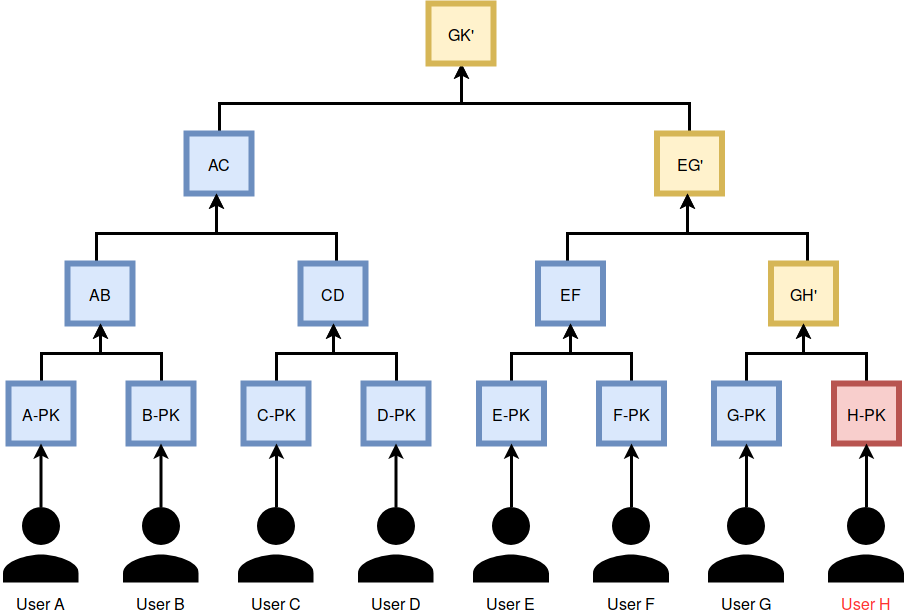
\includegraphics[width=0.8\linewidth]{img/LKH.png}
    \caption{Balanced binary \ac{LKH} and user H leaves the group. Node marked in red is removed from the group. Node marked in yellow require an update and need to be stored locally by any leaf of this node. }
    \label{fig:lkh}
\end{figure*}

Logical Key Hierarchy (\ac{LKH})\cite{wallner1999key} is a \ac{GKMP} that reduces user side storage and rekey transmissions by organizing users keys in a tree hierarchy and maximizing the use of multicast messages. The tree is maintained by a central \textit{Key Distribution Center} (\ac{KDC}). In the work of Wallner \textit{et. al.} \cite{wallner1999key} it is explicitly stated that this trees neither have to be balanced nor binary, but for the sake of simplicity exactly this is assumed. Users (and their respective public keys) are organized at the leafs of the LKH. Each node is composed of a key that is encrypted with its children keys. An encrypted key is known to all leafs related to this node and can, on change of this node, be transmitted in one multicast transmission to all its leafs. The root node summarizes the \ac{GK}. The \ac{GK} is used in the same way as in \ac{GKMP} to secure the group communication. 

While in \ac{GKMP} each user needs to store each members public key to eventually rekey the GK, in \ac{LKH} each user only needs to store $log(n) +1$ keys (path from leaf to root node). Beginning from the bottom, each leaf node could decrypt the next parent node until it arrives at the root node. One other advantage is that many members share the same keys. So it is more efficient to transmit this keys in a multicast setting. \ac{LKH} needs to do $2 log(n)$ multicast transmissions and analogous $2 log(n)$ encryptions on each member leave or join.  Here each updated key in the path from leaf to root node needs to be updated and encrypted two times: One time with the key of right children node and second with the key of the left children node. 

In figure \ref{fig:lkh} user H recently left the group which means, that to ensure forward secrecy, the keys in node $GH$, $EG$ and $GK$ must be updated. The key server will choose a new $GH'$, $EG'$ and $GK'$, encrypts and distributes them in a bottom up fashion starting by $GH'$. $GH'$ is encrypted with user Gs and user Hs public key (G-PK, H-PK) and transmitted to them respective. Next, user E and F receive in a multicast transmission $EG'$, which is encrypted with $EF$ and user G and H receive in a multicast transmission $EG'$ which is now encrypted with the newly established $GH'$ key. Finally, the GK needs to be updated. For the left sub tree $GK'$ is encrypted with $AC$ and transmitted using multicast to the users A, B, C and D. And for the right sub tree $GK'$ is encrypted with $EG'$ to transmitted using multicast to user E, F, G and H. Adding a user to the group follows the same principle. Backward secrecy is implicitly given and not easily removable from this scheme.

\subsection{One-Way Function Trees}
To reduce the transmission and encryption overhead of $2 log(n)$ even further to $log(n)$ other schemes use pseudorandom functions \cite{canetti1999multicast} or one-way functions \cite{sherman2003key} to compute the required keys in the path. This schemes are strongly related to \textit{Merkle Trees}, since each update of the user set will force an update of the root node: The group key.

Each user stores a blinded key for each sibling node in the path to the root node. Starting from his individual key, a user can compute the blinded version of his key. To compute the next parent key, a user utilizes his blinded key, together with the siblings blinded key, which is fed into a one way function to create the key for the parent node. This node needs to be blinded to serve as the input for the next level. In such way the user can compute the needed keys up to the GK. 

Lets assume the same tree layout as in figure \ref{fig:lkh} but assume that user H joined the group. Given a cryptographically secure hash function $h$. First, user H needs to receive the blinded keys, $h(AC)$, $h(EF)$ and $h(G-PK)$ which he stores locally in addition to his own public key $H-PK$. \textit{One-Way Function Trees} (\ac{OWFT}) have the same storage overhead as LKH with $log(n) + 1$.  As already known from LKH, $GH$, $EG$ and $GK$ need to updated. This nodes are computed from their children blinded values using a merging function $m$ which takes two inputs and produces one output. This could for example be the concatenation of both inputs and then applying $h$ to receive a fixed length output value. Starting from the bottom,  $GH'$ is computed as $m(h(G-PK), h(G-PK))$, analogous $EG' = m(h(EF), h(GH'))$ and finally the updated group key $GK' = m(h(AG), h(EG')$. The new blinded keys are distributed to their respective users using one multicast transmission each, reducing the transmission and encryption overhead to $log(n)$. If user H leaves the group, user G must come up with a new random secret that he hashes as placeholder for the previous blinded key of H to compute $GH'$. Thus forward and backward secrecy is enforced.


\subsection{Comparison}  

\begin{table*}[!ht]
\centering
\begin{tabular}{l 		| l 						| l 							| l 						| l 						}
 						& \textbf{Bdrive} & \textbf{\ac{GKMP}}\cite{harney1997group} & \textbf{\ac{LKH}}\cite{wallner1999key} & \textbf{\ac{OWFT}}\cite{sherman2003key} \\%\textbf{\ac{GDH}.1}\cite{steiner1996diffie}\\
\hline
\textbf{inizial share} 																																		\\
keys 					& $nf$	 					& $1$  							& $n-1$  					& $n$	 					\\%& $1$ 			\\
messages (unicast)		& $nf$	  					& $n$ 							& $n(log_2(n) + 1)$ 		& $2n(log_2(n) + 1)$		\\%& $2(n - 1)$	\\
messages (multicast) 	& $nf$	 					& $n$ 							& $log_2(n) + 1$ 			& $n - 2$ 					\\%& $2(n - 1)$ 	\\
encryptions				& $nf$	 					& $f + n$ 						& $f + n -1$				& $f + n -1$				\\%& $f + n$		\\
\hline
\textbf{member join} 																																		\\
keys 					& $f$   					& $1$  							& $3 log_2(n)$				& $log_2(n)$				\\ %& $1$			\\
messages (unicast)		& $f$  						& $1$			 				& $2(n - 1)$				& $n$  						\\ %& $2(n - 1)$	\\
messages (multicast) 	& $f$ 	 					& $1$ 		 					& $2 log_2(n)$				& $log_2(n)$				\\ %& $2(n - 1)$	\\
encryptions				& $f$  						& $f + 1$		 				& $f + 2(log_2(n))$ 		& $f + log_2(n)$			\\ %& $f + 2$	 	\\
\hline
\textbf{member leave}																																		\\
keys 					& $0$						& $1$			  				& $3 log_2(n)$				& $log_2(n)$				\\ %& $1$			\\
messages (unicast)		& $0$						& $n$			 				& $2(n - 1)$ 				& $0$	  					\\ %& $2(n-1)$		\\
messages (multicast)	& $0$						& $n$			 				& $2 log_2(n)$				& $log_2(n)$				\\ %& $2(n-1)$		\\ 
encryptions 			& $0$						& $f + n$ 						& $f + 2 (log_2(n))$ 		& $f + log_2(n)$	 		\\ %& $f+n$			\\
\hline	
\textbf{addition of filekey}																																\\
keys 					& $n$		 				& $0$							& $0$	 					& $0$		 				\\ %& $0$			\\
messages (unicast)		& $n$		 				& $0$	 						& $0$ 						& $0$		 				\\ %& $0$			\\
messages (multicast)	& $n$ 						& $0$ 							& $0$ 						& $0$	 					\\ %& $0$			\\
encryptions				& $n$ 						& $1$ 							& $1$ 						& $1$		 				\\ %& $1$			\\
\hline
\end{tabular}
\caption{Comparison of secure group communication schemes. $n$ donates the number of clients and $f$ the number of file keys. Forward secrecy is ensured in each scheme. Assuming a balanced binary tree as in figure \ref{fig:lkh}}
\label{tab:comparisons}
\end{table*}

Table \ref{tab:comparisons} will compare the discussed schemes against each other regarding number of keys, messages, and encryptions on initialization of the group, when a member joins or leaves and on addition of a new file. 

It is assumed that clients already downloaded the public keys of their group members. Forward secrecy need to be ensured every time a member leaves the group.
Further, messages in table \ref{tab:comparisons} are transmissions that contain a key. There are also meta messages that notify the members about a new file upload or the removal of a member, etc.  They are ignored since they add a constant overhead to all schemes.  If a message could be processed by multiple communication partners it can be transmitted in multicast transmission. In general it is assumped that $f > n$ holds true, since there are usually more files in a share than devices.

Reviewing the performance comparison, Bdrives scheme is not optimal compared to the different approaches. In fact Bdrive has the worst performance on initialization, addition of a filekey and on average also on member join. However, Bdrive has great performance on member leave since client simply do not have to encrypt anymore for the left member.

Each of the schemes have their own strength and weaknesses. \ac{GKMP} has the smallest initialization overhead and \ac{OWFT} the best rekeying overhead. As some could clearly extract from the table that all secure group communication schemes perform better than Bdrive on file upload. Bdrive needs to distribute and encrypt a new filekey $n$ times for each device while any scheme using a \ac{GK} only needs one encryption and one multi cast transmission. 

Under the assumption that a secure cloud storage does not need backward secret, \ac{GKMP} is selected as most suitable candidate. It has great initialization overhead is easily understandable and profits from the fact that no backward secrecy on member join is needed. \ac{LKH} and \ac{OWFT} both have backward secrecy fixed implemented resulting in a bit more worse performance. 